% intro: felix

This section covers existing schema languages and existing approaches to generate UIs from them.
% We compare the schema languages briefly and discuss why JSON schema is the most useful language for our approach.
As our research is of a practical nature, we also consider gray literature such as specifications of schemas or websites.
\subsection{Schema Languages}\label{subsec:schemalanguages}

\textit{Schema languages} are formal languages that specify the structure, constraints, and relationships of data, for example in a database or structured data formats.

As this work is concerned with generating a GUI based on a schema, we need to choose a suitable schema language.
The following sections describe existing schema languages.
We will compare them in section~\ref{sec:evaluation-of-schema-languages} to determine which is the most suitable one for this work.

%paul
\subsubsection{JSON schema}

JSON is a common data-interchange format for exchanging data with web services, but also for storing documents in NoSQL databases, such as MongoDB\@\cite{marrs2017json}.
Because of the popularity of JSON, there is also a demand for a schema language for JSON\@.
One such language is JSON schema~\cite{jsonSchema, jsonschemaJSONSchema}.
Listing~\ref{lst:json-schema-example} shows an example of a JSON schema and listing~\ref{lst:json-example} shows an example of a JSON document that conforms to the schema.

JSON schema has evolved to being the de-facto standard schema language for JSON documents~\cite{baazizi2021empirical}.
Schemas for many popular \cfgfile{} types exist.
\textit{JSON schema store}\cite{schemastoreJSONSchema} is a website that provides over 600 JSON schema files for various use cases.
The supported file types include for example Docker compose or OpenAPI files.
\cite{barbaglia, ChaeronySiffa2022} give further examples of JSON schema used in practice.

JSON and YAML documents are of a similar structure (JSON is a subset of YAML) and JSON schema can be applied to YAML documents too.
Some syntactical details of YAML can, however, not be expressed with JSON schema.

% minye
\begin{lstlisting}[language=json,firstnumber=1,caption={JSON schema example},captionpos=b,label={lst:json-schema-example}]
{
  "$id": "https://example.com
  /person.schema.json",
  "$schema": "https://json-schema.org
  /draft/2020-12/schema",
  "title": "Person",
  "type": "object",
  "properties": {
    "firstName": {
      "type": "string",
      "description": "first name."
    },
    "lastName": {
      "type": "string",
      "description": "last name."
    },
    "age": {
      "description": "Age",
      "type": "integer",
      "minimum": 0
    }
  }
}
\end{lstlisting}


\begin{lstlisting}[language=json,firstnumber=1,caption={JSON example for the schema in listing}~\ref{lst:json-schema-example},captionpos=b,label={lst:json-example}]
{
  "firstName": "John",
  "lastName": "Doe",
  "age": 21
}
\end{lstlisting}

% felix
\subsubsection{XSD and DTD}
For XML the two de-facto standard schema languages are Document Type Definition (DTD)\cite{dtd_spec} and XML Schema Definition (XSD)\cite{xsd_spec}.
XSD is the newer and more expressive format and in large parts replaces and supersedes the more limited format DTD\cite{dtd_vs_xsd}.
It is recommended by W3C as a schema language for XML documents\cite{xsd_spec}.
Multiple other schema languages have been proposed and developed but are relatively unknown compared to XSD\cite{xml_schemas_1,xml_schemas_2}.

\subsubsection{Other schema languages} %Minye
We also consider the following schema languages:
\begin{enumerate}[label=(\alph*)]
    \item CUE (Configure, Unify, Execute)\cite{cuelang} is a data validation and configuration language, which can be used with various data formats, such as JSON and YAML (it is a superset of both).
    It has several use cases, especially in configuration and data validation.
    \item Apache Avro~\cite{Apache-Avro} is an open-source project that provides data serialization and data exchange services for Apache Hadoop.
    It uses a JSON-based schema language.
    \item JSON Type Definition (JTD)~\cite{rfc8927} is a schema language for JSON documents, which is significantly simpler than JSON schema.
    \item Type Schema~\cite{Kappestein_2023} is a schema language for JSON documents, similar to JSON Type Definition but using a different syntax.
    \item GraphQL schema language~\cite{graphQL} is a schema language for GraphQL APIs.
    \item Protocol Buffers~\cite{protobufProtocolBuffers} is a language for data serialization by Google.
\end{enumerate}

We do not consider any graphical modeling languages, such as UML or ER diagrams, as they are not text-based.
Although they can be converted to text-based formats, their main purpose is to model data structures and relationships between them.
We also do not consider any ontology languages, such as OWL or RDF Schema, as they are not intended for data validation but rather for knowledge representation.
Future work could investigate if such languages are also useful for our use case.
Finally, we do not consider any programming languages as schema languages.
Technically, programming languages can be used to define data structures and constraints, but they are not intended for this purpose, and it would be very challenging to generate a GUI from them.

\subsection{Existing Approaches}\label{subsec:existing-approaches}
% felix
Our work focuses on assisting users in creating and maintaining \cfgfiles{} so that they are valid and adhere to a predefined schema.

%There exist several approaches that attempt to make maintaining \cfgfiles easier for the user.
%Most of these approaches depend on the schema of the configuration file to be known.
There exist techniques to validate \cfgfiles{} against a schema~\cite{JSON_schema_vailidation,JSONValidation,baeldung_2023}.
Usually, schema validation is done only internally, e.g., by web services or libraries.
However, there exist also approaches that use the schema to assist the user in creating and maintaining \cfgfiles.
IDEs, such as Visual Studio Code or IntelliJ IDEA, can validate \cfgfiles{} against a schema and provide the user with error messages.
Those IDEs provide also other features, such as auto-completion, syntax highlighting, and tooltips.
However, they typically do not provide a graphical user interface (GUI) for editing the \cfgfiles{} based on the schema.


\subsubsection{Form generation}\label{subsubsec:schema-to-gui}
% minye and felix and paul

Related to our work are approaches that generate a GUI from a schema.
This section covers form generators, i.e., approaches that generate a web form from a schema.
Such forms can assist the user in a multitude of ways, such as by tooltips, auto-completion (Figure~\ref{fig:gui_advantage_autocomplete}) and dropdown menus (Figure~\ref{fig:gui_advantage_choiceselection}).
By inherently adhering to the schema structure (in most cases), editing data with such GUIs significantly reduces configuration mistakes caused by the user.
Users who are not very familiar with the configuration schema profit most from the GUI assistance, but even experienced users benefit from it.

\begin{figure}[htb]
\centering
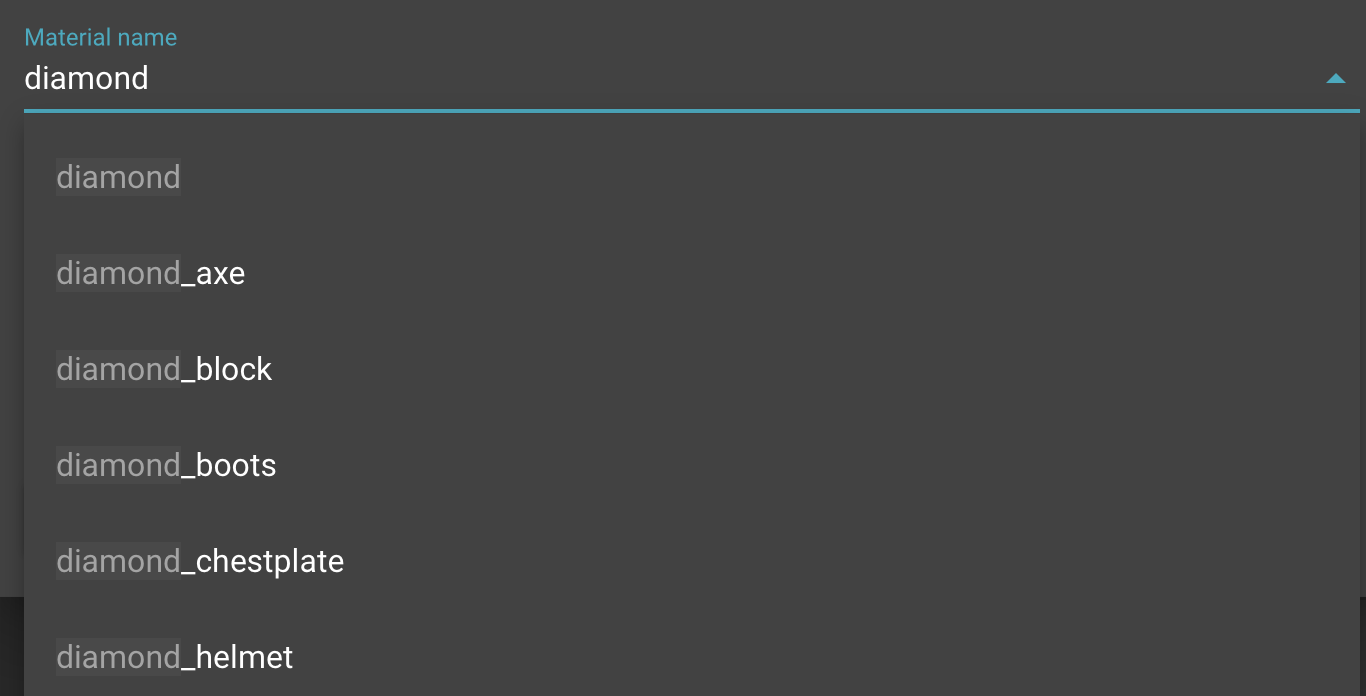
\includegraphics[width=2.5in]{figures/gui_advantage_autocomplete}
\caption{Auto-Completion}
\label{fig:gui_advantage_autocomplete}
\end{figure}

\begin{figure}[htb]
\centering
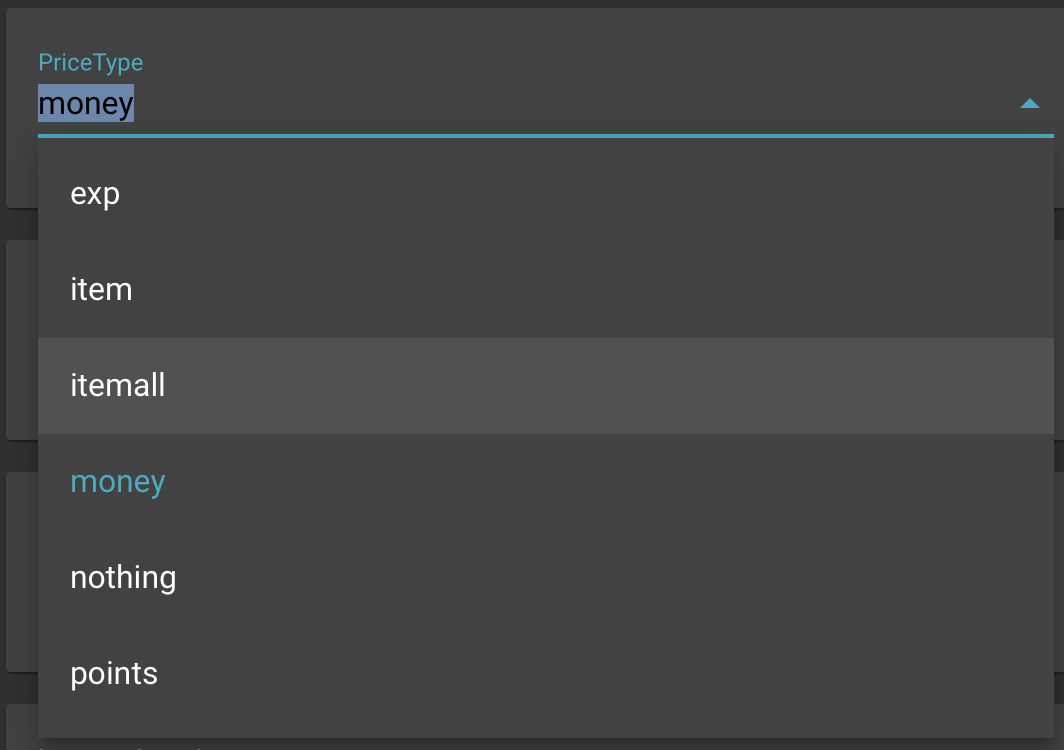
\includegraphics[width=2.5in]{figures/gui_advantage_choiceselection}
\caption{Choice Selection}
\label{fig:gui_advantage_choiceselection}
\end{figure}

%paul
There exist various approaches that generate web forms from a schema, for different frontend frameworks, e.g.,
\textit{React JSON Schema Form}\cite{githubGitHubRjsfteamreactjsonschemaform},
\textit{Angular Schema Form}\cite{githubGitHubJsonschemaformangularschemaform},
\textit{Vue Form Generator}\cite{githubGitHubVuegeneratorsvueformgenerator},
\textit{JSON Forms}\cite{jsonformsMoreForms},
\textit{JSON Editor}\cite{jsoneditoronlineJSONEditor}, and
\textit{JSON Form}\cite{githubGitHubJsonformjsonform}.
Those approaches are all based on JSON schema and generate a form that can be filled out by the user and
the resulting JSON document is validated against the schema.
If the user enters invalid data, the form shows an error message.
The generated forms usually have a specific component for each type of data, e.g.\ a text field for strings or a number field for numbers,
similar to our approach.
Figure~\ref{fig:jsonforms} shows an example of a generated form using JSON Forms.

Those techniques, however, only provide the GUI for editing the data, but not a text-based editor.
A text-based editor is useful, especially for experienced users, who prefer to edit the data directly.
Also, these techniques do not provide a way to edit the schema itself, but only the data.
The most significant limitation of all except the last two of the given approaches is that they also require a ``UI schema'' in addition to the JSON schema, which is used to configure the generated form.
While these configurations can be used to customize the generated form, they also need to be created and maintained by the schema author.
Consequently, those approaches cannot be used to generate a GUI for any arbitrary schema, but manual effort is required to create the UI schema.

\begin{figure}[htb]
    \centering
    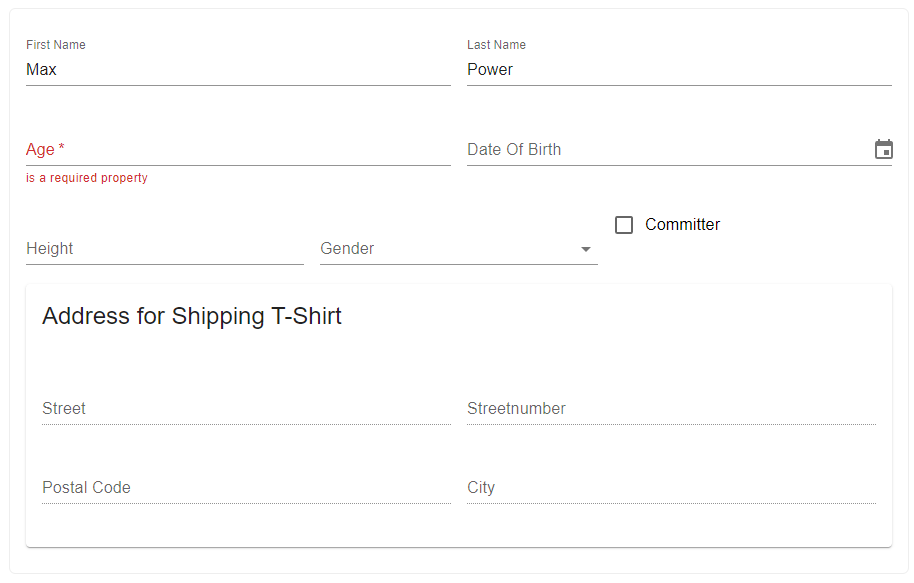
\includegraphics[width=2.5in]{figures/jsonforms}
    \caption{JSON Forms, example for a generated form}
    \label{fig:jsonforms}
\end{figure}

Adamant~\cite{siffa2022adamant} is a JSON-schema based form generator specifically designed for scientific data.
It is similar to our approach in that it generates a GUI from a JSON schema and also allows to edit and create JSON schema documents
and differentiates between a schema edit mode and a data edit mode.
It supports a subset of JSON schema, which is sufficient for many use cases.
In addition to that, it supports the extraction of units from the description of a field, which is helpful for scientific data.
Figure~\ref{fig:adamant} shows an example in the schema edit mode.
%Adamant differs to \toolname{} in that it does not provide a text-based editor for the schema and that it is specifically designed for scientific data,
%while our approach is more general.
Limitations of Adamant are first, it does only support a subset of JSON schema, which is sufficient for many use cases, but not for any arbitrary schema.
Second, it does not provide a text-based editor for neither the schema nor the data.
Finally, it is specifically designed for scientific data, which makes it less suitable for other use cases, especially large and complex schemas.

\begin{figure}[htb]
    \centering
    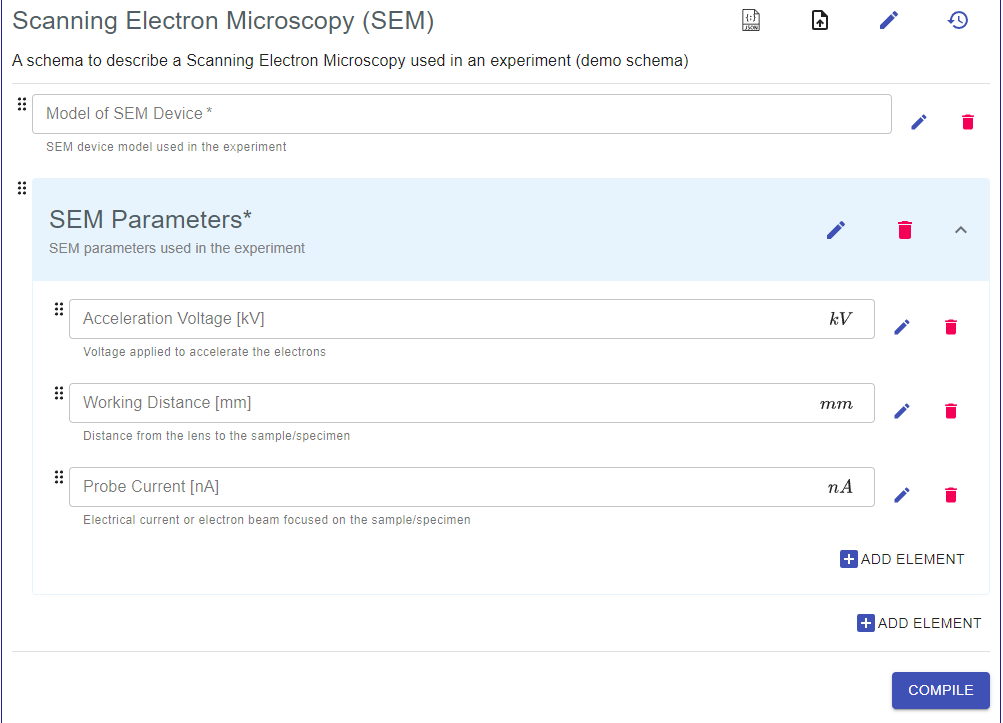
\includegraphics[width=2.5in]{figures/adamant}
    \caption{Adamant, example for a form in edit mode}
    \label{fig:adamant}
\end{figure}


\subsubsection{Schema editors}\label{subsubsec:schema-editors}
In \toolname{} we aim to provide a GUI for both editing \cfgfiles{} and editing the schema.
For the latter, there exist several so-called schema editors, which are tools for creating and editing schemas that are
either text-based or graphical (or both).

\textit{JSON Editor Online}\cite{jsoneditoronlineJSONEditor} is a web-based editor for JSON schemas and JSON documents.
It divides the editor into two parts, where one part can be used to edit the schema and the other part can be used to edit a JSON document,
which is validated against the schema.
The editor provides various features, such as syntax highlighting and highlighting of validation errors (Figure~\ref{fig:jsoneditoronline}).
It provides a text-based or tree-based view for editing the JSON documents.
For simple objects that are not further nested, it provides also a table-based view (Figure~\ref{fig:jsoneditoronline_table}).
However, the features of the editor are very limited.
For example, it does not provide any assistance for the user, such as tooltips or auto-completion.
For new documents, it does not show the properties of the schema, so the user has to know the schema beforehand.

There also exists a variety of schema editors that are paid software, such as \textit{Altova XMLSpy}\cite{altovaEditorXMLSpy},
\textit{Liquid Studio}\cite{liquidtechnologiesJSONSchema}, \textit{XML ValidatorBuddy}\cite{xmlbuddyEditorValidator},
\textit{JSONBuddy}\cite{jsonbuddyJSONSchema}, \textit{XMLBlueprint}\cite{xmlblueprintEditorXMLBlueprint},
and \textit{Oxygen XML Editor}\cite{oxygenxmlCompleteSolution}.
Those are editors for XML or JSON schema, mostly with a combination of text-based and graphical views.
These tools are not web-based and not open-source.
Furthermore, they do not focus on editing a JSON document based on a schema,
but rather only on editing the schema itself.
\begin{figure}[htb]
	\centering
	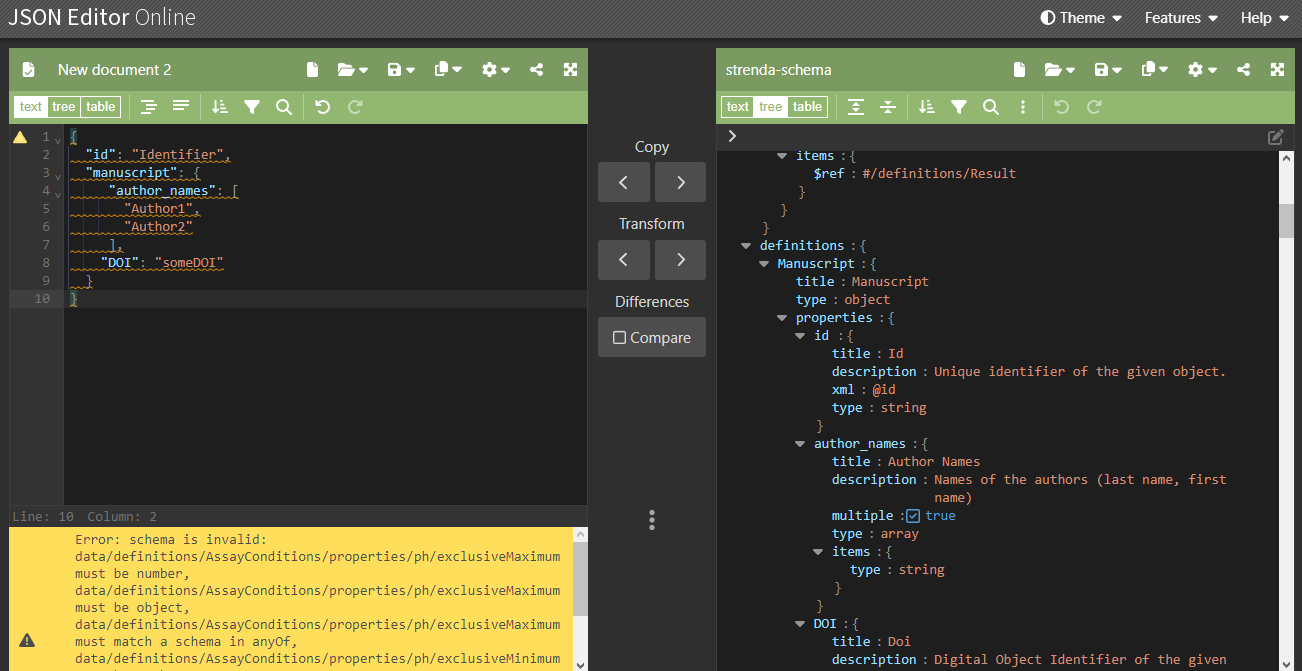
\includegraphics[width=3in]{figures/jsoneditoronline}
	\caption{JSON Editor Online}
	\label{fig:jsoneditoronline}
\end{figure}
\begin{figure}[htb]
	\centering
	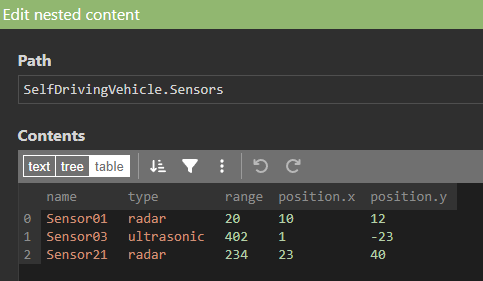
\includegraphics[width=3in]{figures/jsoneditoronline-table}
	\caption{JSON Editor Online, table view}
	\label{fig:jsoneditoronline_table}
\end{figure}


\subsubsection{Schema visualization}\label{subsubsec:schema-visualization}
Generating a GUI from a schema is related to schema visualization, for which several techniques exist~\cite{Frasincar2006, SILVA201928, 10.1145/1317353.1317362, 1173142}.
However, the focus of schema visualization is on providing a static visual representation of the schema
and not on providing a GUI for editing the schema.
Thus, we do not consider schema visualization approaches in this work.
However, future work could investigate how such techniques could be embedded in our approach.


\section{Evaluation of Schema Languages}\label{sec:evaluation-of-schema-languages}


We evaluate the schema languages mentioned in section~\ref{subsec:schemalanguages} to determine which is the most suitable one for this work.


\subsection{Evaluation criteria}\label{subsec:evaluation-criteria} % evaluation by paul, some criteria ideas by felix

Ideally, the schema language of \toolname{} is both popular and supported by numerous tools and libraries as well as expressive enough to express the features we need.
We use the following criteria and metrics:
\begin{enumerate}
% metric: Stackoverflow question # with schema language as tag
    \item \textbf{Practical usage} --- Ideally our approach uses a schema language that already known by many developers.
    As indicator of the practical usage we use the approximate search results on stackoverflow.com as metric.
    We acquire the results by querying the google search engine with the name of the schema language and ``site:stackoverflow.com'', which limits the search results to stackoverflow.com.
    This metric might also correlate with the complexity of the schema language as a more complex to use schema language will likely lead to more questions asked on the site.
    Nevertheless, we assume that a significantly higher number of results indicates that a language is more known than others.

    Additionally, we investigate how well the schema languages are supported by IDEs and code libraries:
    \begin{enumerate}
        \item \textit{Tool support} --- We used the 10 most popular IDEs\cite{mostpopularides} and checked if the IDE supports the schema language either natively or by a plugin.
        Support here means that either the IDE is capable of validating documents against a schema in the schema language or supports creating schema files, e.g., by using syntax highlighting for the schema language.
        % # node modules with schema language keyword....
        \item \textit{Library support} --- As we implement a web-based tool, we JavaScript or TypeScript bases tools are helpful for our approach, e.g., so we can reuse a package for schema validation.
        We investigate the number of node modules exist that are related to the schema languages by querying the node module search on \url{www.npmjs.com} with the name of the schema language.

    \end{enumerate}

    % # of cases fulfilled from below
    \item \textbf{Expressiveness} --- We evaluate how expressive each of the schema languages are, i.e., what possible constructs the language is able to express.
    We define eight requirements on the language features that we consider helpful for our approach.
    The number of requirements a schema language fulfills is our metric that indicates how expressive the language is.
    Table~\ref{tab:comparison} reports the results.
    The nine requirements are:
    \begin{enumerate}
        \item \textit{Simple types} --- This is fulfilled if the schema language provides the possibility to define simple data types, at least strings, numeric types, and a boolean type.
        This is a fundamental feature for our approach.
        \item \textit{Complex types} --- This is fulfilled if the schema language provides the possibility to define complex data types, at least records and arrays.
        This is crucial feature for our approach as configuration files are often structured data rather than plain key-value pairs.
        \item \textit{Descriptions} --- This is fulfilled if the schema language provides the possibility to add descriptions to fields.
        This is helpful in a schema-to-GUI approach as the description can be shown to the user, providing potential helpful information on how a field should be filled.
        \item \textit{Examples} --- This is fulfilled if the schema language provides the possibility to add example values.
        This is helpful in our approach as the example values can serve as placeholders in the GUI editor.
        \item \textit{Default values} --- This is fulfilled if the schema language provides the possibility to add default values which are assumed in an absence of a value.
        This often helpful information can be displayed to the user or used as placeholder values.
        \item \textit{Optional values} --- This is fulfilled if the schema language provides the possibility to declare values as optional or required.
        Often it is not necessary to provide all values in a configuration file, so it is helpful to mark fields as required or optional in the GUI editor.
        \item \textit{Constraints} --- This is fulfilled if the schema language provides the possibility to constrain values of fields, e.g., maximum length of strings.
        To be exact, for this evaluation we required that at least two of the following constrained can be expressed by the schema language:
        \begin{itemize}
            \item The length of strings can be limited.
            \item The range of numeric types can be limited, e.g., to only positive values.
            \item The valid values of a field can be restricted to a finite amount of values (enumeration).
            \item The format of a string field can be constrained to a certain pattern.
        \end{itemize}
        This is a helpful feature for our approach as often not all possible values are valid for specific fields in configuration files.
        \item \textit{Conditions} --- This is fulfilled if the schema language provides the possibility to define conditional dependencies between fields.
        This is a advanced feature that is helpful because it allows to express for example that a particular field must be given only if another field has a specific value.
        \item \textit{References} --- This is fulfilled if the schema language provides the possibility to define reusable subschemas that can be referenced in other parts of the schema.
        This is often useful in practice to reuse common data structures.

    \end{enumerate}

    %\item \textbf{Support for XML, YAML, or JSON} ---

    % For our approach we aim to use the same or at least a very similar editor for both editing the actual \cfgfiles and the schema files. Consequently, the schema language should be a subset of the language that the \cfgfiles are written in, i.e. the document language. For example JSON schema files are JSON files and JSON schema is used to validate JSON files, so here this criteria is fulfilled. In constrast, DTD is a schema language for validating XML files but a DTD file is not a valid XML file.

\end{enumerate}


    \begin{table*}[]
    \centering
    \caption{Evaluation of different schema languages\label{tab:all}}
        \begin{tabular}{@{}lrrrr@{}}
        \toprule
        \textbf{Schema language} &
          \textbf{\# Search results } &
          \textbf{IDE support} &
          \textbf{\# Node packages} &
          \textbf{Expressiveness} \\ \midrule
        JSON schema &
          245.000 &
          8 / 10 &
          4.536 & 9 /9 \\
        XSD & 151.000 & 8 / 10 & 116 & 8 / 9 \\
        DTD & 69.700 & 9 / 10 & 34 & 6 / 9 \\
        CUE & 10.500 & 4 / 10 & 97 &   8 / 9 \\
        Avro & 20.000 & 8 / 10 & 211 &  5 / 9 \\
        JSON Type Definition (JTD) &  109 & 0 / 10 &  17 & 5 / 9 \\
        TypeSchema &  8.450 & 0 / 10 & 5 & 8 / 9 \\
        protobuf &  44.800 & 9 / 10 & 1.210 & 4 / 9 \\
        GraphQl schema & 31.000 & 7 / 10 & 1.509 & 6 / 9\\ \bottomrule
        \end{tabular}
    \end{table*}
    %\label{fig:my_label}
%\end{figure}

% IDE                | JSON schema | XSD | DTD | CUE | Avro | protobuf | GraphQL schema |
% Visual Studio      | yes         | yes | yes | x   | yes  | yes      | yes            |
% Visual Studio Code | yes         | yes | yes | yes | yes  | yes      | yes            |
% Eclipse            | yes         | yes | yes | x   | yes  | yes      | x              |
% pyCharm            | yes         | yes | yes | yes | yes  | yes      | yes            |
% Android Studio     | yes         | yes | yes | yes | yes  | yes      | yes            |
% IntelliJ           | yes         | yes | yes | yes | yes  | yes      | yes            |
% NetBeans           | x           | yes | yes | x   | x    | yes      | x              |
% RStudio            | x           | x   | x   | x   | x    | x        | x              |
% Atom               | yes         | x   | yes | x   | yes  | yes      | yes            |
% Sumblime Text      | yes         | yes | yes | x   | yes  | yes      | yes            |
% ======================================================================================|
%                    | 8 / 10      | 8   | 9   | 4   | 8    | 9        | 7              |

\begin{table*}
    \centering
    \caption{Comparison of expressiveness of different schema languages
    \label{tab:comparison}}
    \begin{tabular}{@{}llllllllllr@{}}
        \toprule
        \textbf{Schema language} &
          \thead{Simple \\ types} &
          \thead{Complex \\ types} &
          \thead{Descriptions} &
          \thead{Example \\ values} &
          \thead{Default \\ values} &
          \thead{Optional \\ values} &
          \thead{Constraints} &
          \thead{Conditions}  &
          \thead{References}  &
          \thead{Result}\\ \midrule
        JSON schema &
          \checkmark &
          \checkmark &
          \checkmark &
          \checkmark &
          \checkmark &
          \checkmark &
          \checkmark &
          \checkmark &
          \checkmark & 9 / 9\\
        XSD &
          \checkmark &
          \checkmark &
          \checkmark &
          x &
          \checkmark &
          \checkmark &
          \checkmark &
          \checkmark &
          \checkmark & 8 / 9 \\
        DTD &
         \checkmark &
         \checkmark &
         x &
         x &
         \checkmark &
         \checkmark &
         x &
         \checkmark &
         \checkmark & 6 / 9\\
        CUE &
         \checkmark &
         \checkmark &
         \checkmark &
         \checkmark &
         x &
         \checkmark &
         \checkmark &
         \checkmark &
         \checkmark & 8 / 9\\
        Avro &
         \checkmark &
         \checkmark &
         x &
         x &
         \checkmark &
         \checkmark &
         x &
         x &
         \checkmark & 5 / 9\\
        JTD &
         \checkmark &
         \checkmark &
         x &
         x &
         x &
         \checkmark &
         x &
         \checkmark &
         \checkmark & 5 / 9\\
        TypeSchema &
         \checkmark &
         \checkmark &
         \checkmark &
         x &
         \checkmark &
         \checkmark &
         \checkmark &
         \checkmark &
         \checkmark & 8 / 9\\
        protobuf &
            \checkmark &
            \checkmark &
            x &
            x &
            x &
            \checkmark &
            x &
            x &
            \checkmark & 4 / 9 \\
        GraphQL schema &
         \checkmark &
         \checkmark &
         \checkmark &
         x &
         \checkmark &
         \checkmark &
         x &
         x &
        \checkmark & 6 / 9\\
          \bottomrule
    \end{tabular}
\end{table*}

% paul
\subsection{Evaluation results}\label{subsec:evaluation-results}

Tables~\ref{tab:all} and~\ref{tab:comparison} show the results of our evaluation.
We come to the conclusion that JSON schema is sufficiently popular and expressive that we choose to use it as the schema language for our approach.
The other schema languages are either less expressive or less popular.
This result is in line with the work of Baazizi et al.~\cite{baazizi2021empirical}, who also found over 80.000 JSON schema files on GitHub,
and with their claim that JSON schema is the de-facto standard for JSON schema languages.

% paul

%\subsection{Schema inference}\label{subsec:schema-inference}
%
%Schema inference is the process of deriving a schema from existing data.
%For our use case, this means inferring JSON schema from JSON documents.
%Frozza et al.~\cite{8424731} and Klettke et al.~\cite{klettke} present algorithms for JSON schema inference from JSON data of NoSQL data storages.
%Baazizi et al.\cite{Baazizi2019} also investigate schema inference from massive data sets but their approach uses its own type system rather than JSON schema.
%
%In our tool we only aim to infer a schema from a single sample, as an optional assisting feature for our users, for which various libraries exist~\cite{githubGitHubJsonsystemspublic, githubGitHubSaasquatchjsonschemainferrer, probst_siegel_2023}.
